\documentclass[a4paper, 12pt]{article}

\input{~/Desktop/Studia/LaTeX/setup_eng.tex}
\author{Wojciech Orłowski}
\title{Solving Schrodinger equation in two dimensional \\ anisotropic harmonic oscillator using Gallerkin method}

\begin{document}
\maketitle

\section*{Introduction}

The main goal of laboratory class is calculate energies and wavefunctions of anisotropic quantum harmonic oscillator in two dimensions.
We can interpret such a system as a single electron trapped inside two-dimensional quantum dot.
We can easily get accurate values using Gallerkin method in gaussian function basis.

\section*{Results}

\subsection*{First task}

The first task was to construct correct basis.
We can ensure that basis is build properly by plotting some of basis functions (fig. \ref{fig:basis}).

\begin{figure}[h]
    \begin{center}
        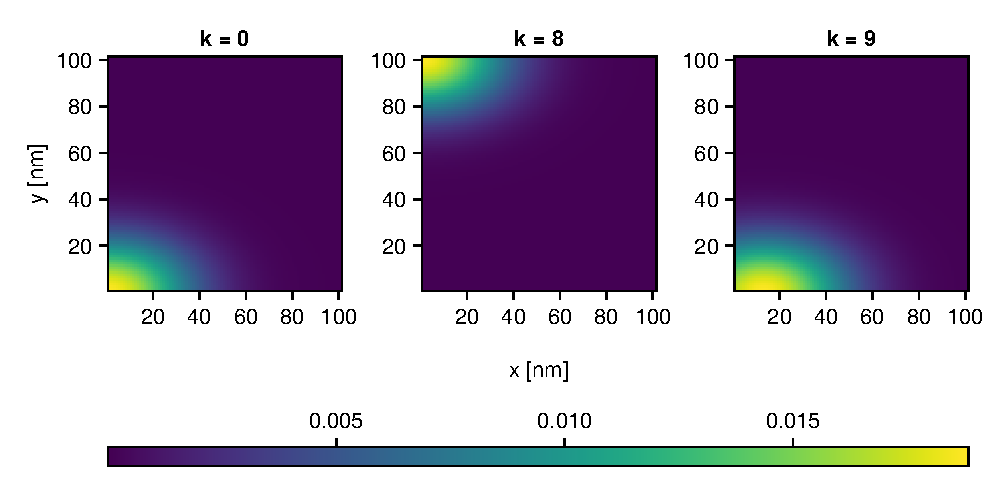
\includegraphics[width=0.95\textwidth]{../ploters/plots/basis_funcs.pdf}
    \end{center}
    \caption{Few basis functions used in calculations.}
    \label{fig:basis}
\end{figure}

\subsection*{Second task}

The generalized eigenequation was solved using C++ numerical library - \texttt{Eigen3}.
The class \texttt{GeneralizedSelfAdjointEigenSolver} was used as the main solver.
Whole code has been published at \href{https://github.com/OrlowskiWojtek/QuantumTransport}{GitHub} repository.

\subsection*{Third task}

For $\Delta x = 1$ nm system has been solved and first six wavefunctions has been plotted (fig. \ref{fig:wavefunctions}). 

\begin{figure}[h]
    \begin{center}
        \includegraphics[width=0.95\textwidth]{../ploters/plots/wavefunctions.pdf}
    \end{center}
    \caption{Energies and wavefunctions of ground state and five excited states of quantum oscillator $h\omega_x$ = 80 meV, $h\omega_y$ = 200 meV.}
    \label{fig:wavefunctions}
\end{figure}

We can see that system is excited in both directions, according to energy of excited state.
In higher states the energy is not as accurate as for the first states.

\newpage
\subsection*{Fourth task}

Energies of first ten states were plotted versus changing frequency $\hbar\omega_x$ of oscillator (fig. \ref{fig:energies}).

\begin{figure}[h]
    \begin{center}
        \includegraphics[width=0.95\textwidth]{../ploters/plots/energies_10_states.pdf}
    \end{center}
    \caption{Energies of first ten states plotted against frequency of oscillator in $x$ direction.}\label{fig:energies}
\end{figure}

On this plot we can see energy jumps which is connected to excitement in other direction.
Ground state energy is simple line.

\newpage
\subsection*{Fifth task}
On last task we were supposed to find such a frequency of oscillator in $y$ direction so the first 5 states are excited in $x$ direction.
Energy in $y$ direction was arbitrary chosen to be 350 meV (fig. \ref{fig:wavefunctions_high}).

\begin{figure}[h]
    \begin{center}
        \includegraphics[width=0.95\textwidth]{../ploters/plots/wavefunctions_high_omegay.pdf}
    \end{center}
    \caption{Energies and wavefunctions of ground state and five excited states of quantum oscillator $h\omega_x$ = 80 meV, $h\omega_y$ = 350 meV.}
    \label{fig:wavefunctions_high}
\end{figure}

If we would like to have even more first excitements in $x$ direction we should increase frequency value in $y$ direction.
Comparing received data with STM maps we can clearly see that measured gate resembles states of quantum harmonic oscillator.

\section*{Summary}

Galerkin method is a powerful source of information for systems with one electron when we can easily calculate needed values analitycally ($\vb{H}$, $\vb{S}$ matrices).
In this case it helped us to understand two dimensional harmonic oscillators.
Many quantum systems can be interpreted as such oscillators.

\end{document}
